\begin{maintask}{1-C}
  \subsection*{課題内容}
  LAN内のTCP echoサーバに接続し，送信した文字列がそのまま返ってくることを，IPv4・IPv6の双方で確認した．

  \subsection*{実験方法}
  \begin{enumerate}
    \item 1つ目のターミナルでキャプチャを開始
      \begin{minted}{zsh}
        tcpdump -i eth1 -s 0 -w C.pcap 'not port 4200'
      \end{minted}

    \item キャプチャ中に，別のターミナルでtelnetを実行し，適当な文字列を入力して返信を確認したのち，Ctrl+]，quitで終了する．IPv4とIPv6の双方で行う．
      \begin{minted}{zsh}
        (IPv4) telnet 172.28.0.200 echo
        (IPv6) telnet 2001:2f8:40:11da::200 echo
      \end{minted}

    \item キャプチャ側でCtrl-Cを押し，pcapをダウンロードしてWiresharkで開く
  \end{enumerate}

  \subsection*{結果}
  tcpdumpの実行結果と，IPv4・IPv6のtelnetの実行結果をそれぞれ
  出力\ref{out:tcpdump_c}，
  出力\ref{out:telnet_v4}，
  出力\ref{out:telnet_v6}
  に示した．

  \begin{termout}[H]
    \caption{tcpdump の実行結果}\label{out:tcpdump_c}
    \begin{minted}{zsh}
    guest@host82:~$ tcpdump -i eth1 -s 0 -w C.pcap 'not port 4200'
    tcpdump: listening on eth1, link-type EN10MB (Ethernet), capture size 262144 bytes
    ^C500 packets captured
    502 packets received by filter
    0 packets dropped by kernel
    \end{minted}
  \end{termout}

  \begin{termout}[H]
    \caption{telnet(IPv4) の実行結果}\label{out:telnet_v4}
    \begin{minted}{zsh}
    guest@host82:~$ telnet 172.28.0.200 echo
    Trying 172.28.0.200...
    Connected to 172.28.0.200.
    Escape character is '^]'.
    hello
    hello
    world
    world
    ^]
    telnet> quit
    Connection closed.
    \end{minted}
  \end{termout}

  \begin{termout}[H]
    \caption{telnet(IPv6) の実行結果}\label{out:telnet_v6}
    \begin{minted}{zsh}
    guest@host82:~$ telnet 2001:2f8:40:11da::200 echo
    Trying 2001:2f8:40:11da::200...
    Connected to 2001:2f8:40:11da::200.
    Escape character is '^]'.
    hoge
    hoge
    huga
    huga
    ^]
    telnet> quit
    Connection closed.
    \end{minted}
  \end{termout}

  \begin{figure}[htbp]
    \centering
    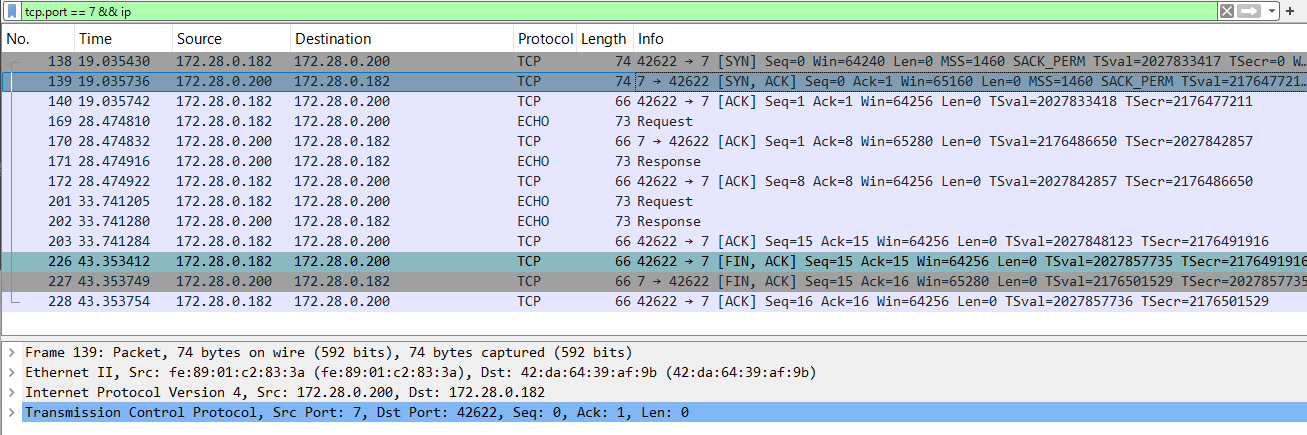
\includegraphics[width=0.98\columnwidth]{fig/wireshark_c_v4.png}
    \caption{IPv4のTCP echo通信をWiresharkで読み取った結果}
    \label{fig:ws_c_v4}
  \end{figure}

  \begin{figure}[htbp]
    \centering
    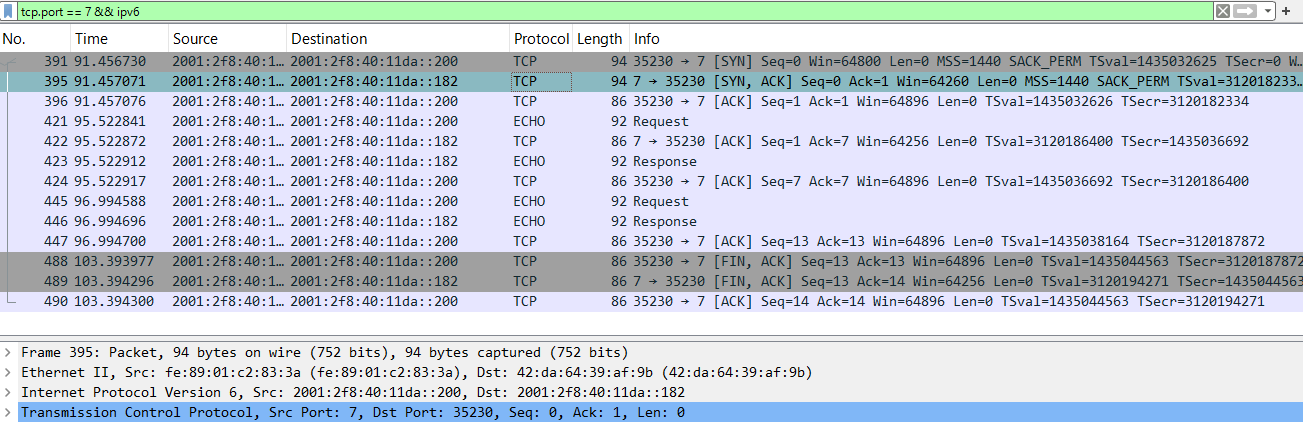
\includegraphics[width=0.98\columnwidth]{fig/wireshark_c_v6.png}
    \caption{IPv6のTCP echo通信をWiresharkで読み取った結果}
    \label{fig:ws_c_v6}
  \end{figure}

  \begin{figure}[htbp]
    \centering
    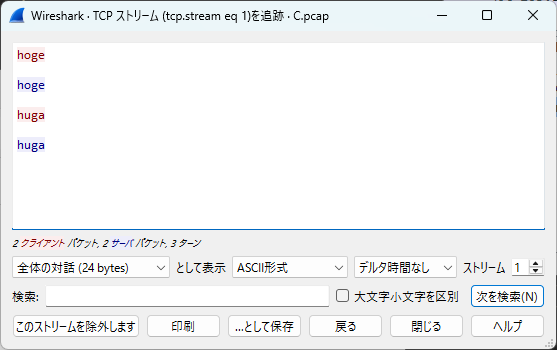
\includegraphics[width=0.7\columnwidth]{fig/wireshark_c_stream.png}
    \caption{TCPストリームの追跡結果(IPv6)}
    \label{fig:ws_c_stream}
  \end{figure}

  IPv4では，出力\ref{out:telnet_v4}のとおり，入力したhelloとworldがそれぞれそのままサーバから返ってきた．図\ref{fig:ws_c_v4}では，まずNo.138のSYN，No.139のSYN/ACK，No.140のACKにより，TCPの3ウェイハンドシェイクで接続が確立している．続いて，No.169でhelloを含むECHOのRequest（データ長7バイト）がクライアント(172.28.0.182)からサーバ(172.28.0.200)へ送られ，サーバはNo.170でACKを返したのち，No.171で同じ7バイトのResponseを返している．これをクライアントがNo.172でACKしている．worldについても同様に，No.201のRequest，No.202のResponse，No.203のACKの順にやり取りされている．データ長が7バイトであるのは，helloの5バイトに，Enterで付加される改行コード(CR LF)の2バイトが加わっているためと考えられる．最後に，クライアントがquitで接続を終了した際，No.226のFIN/ACK，No.227のFIN/ACK，No.228のACKにより接続が閉じられている．

  IPv6でも，出力\ref{out:telnet_v6}のとおり，入力したhogeとhugaがそのまま返ってきた．図\ref{fig:ws_c_v6}では，クライアント(2001:2f8:40:11da::182)とサーバ(2001:2f8:40:11da::200)の間で，IPv4と同じ手順で通信が行われている．No.391のSYN，No.395のSYN/ACK，No.396のACKで接続が確立し，No.421のRequestに対してNo.422のACK，No.423のResponse（データはいずれも6バイト），No.424のACKが続く．hugaについても，No.445のRequest，No.446のResponse，No.447のACKの順にやり取りされている．接続の終了は，No.488のFIN/ACK，No.489のFIN/ACK，No.490のACKである．図\ref{fig:ws_c_stream}のTCPストリームの追跡(IPv6)では，hogeとhugaが送信側・受信側の双方で一致して表示され，全体の対話は24バイトであった．これは，6バイトのデータが4回（送信2回，受信2回）やり取りされた合計と一致する．

  IPv4とIPv6を比べると，TCPの手順（3ウェイハンドシェイク，データの送受信，FINによる終了）は同じである．一方で，SYNパケットの長さはIPv4の74バイトに対してIPv6では94バイトと20バイト大きい．これはIPヘッダが20バイトから40バイトになったためである．また，SYNに含まれるMSSの値も，IPv4の1460に対してIPv6では1440と20バイト小さく，同じ理由で説明できる．なお，echoサービスのポート番号は7であり，いずれの通信もサーバ側のポートは7である．
\end{maintask}
